% core TikZ only; no extra library beyond the paper preamble is required.
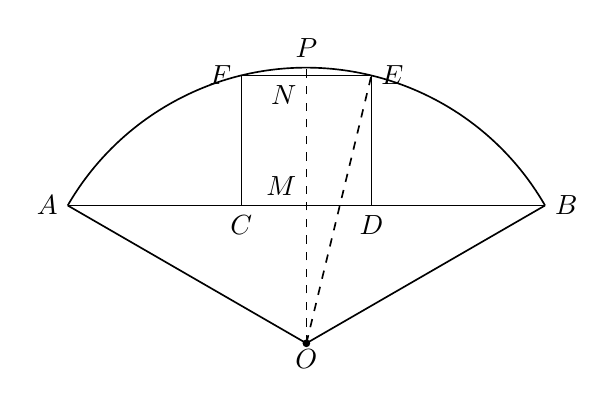
\begin{tikzpicture}[x=1cm,y=1cm,line width=.6pt,font=\normalsize]
\coordinate (O) at (0,0);
\coordinate (A) at (-3.031089,1.75);
\coordinate (B) at (3.031089,1.75);
\coordinate (M) at (0,1.75);
\coordinate (C) at (-0.825615,1.75);
\coordinate (D) at (0.825615,1.75);
\coordinate (P) at (0,3.5);
\coordinate (N) at (0,3.401229);
\coordinate (F) at (-0.825615,3.401229);
\coordinate (E) at (0.825615,3.401229);
\draw (B) arc[start angle=30,end angle=150,radius=3.5cm];
\draw (A)--(B);
\draw (A)--(O);
\draw (B)--(O);
\draw (F)--(C);
\draw (E)--(D);
\draw (F)--(E);
\draw[dashed] (O)--(P);
\draw[dashed] (O)--(E);
\node[left] at (A) {$A$};
\node[right] at (B) {$B$};
\node[below=2pt,inner sep=0pt] at (O) {$O$};
\node[below] at (C) {$C$};
\node[below] at (D) {$D$};
\node[left] at (F) {$F$};
\node[right] at (E) {$E$};
\node[above] at (P) {$P$};
\node[above left] at (M) {$M$};
\node[below left] at (N) {$N$};
\fill (O) circle[radius=1.4pt];
\end{tikzpicture}
